%!TEX root = Presentation-Thoma.tex
\section{Taxonomie}
\subsection{Taxonomie}

\begin{frame}{Taxonomie}
    \begin{enumerate}
        \item Klassen
        \item Pixelzugehörigkeit
        \item Daten
        \item Betriebsart
    \end{enumerate}
\end{frame}

\begin{frame}{Taxonomie: Klassen}
    \begin{enumerate}
        \item Welche Klassen gibt es?
        \item Gibt es eine \textbf{void} Klasse?
    \end{enumerate}
\end{frame}

\begin{frame}{Taxonomie: Pixelzugehörigkeit}
    \begin{center}
        Zu wie vielen Klassen kann ein Pixel gehören?\\

        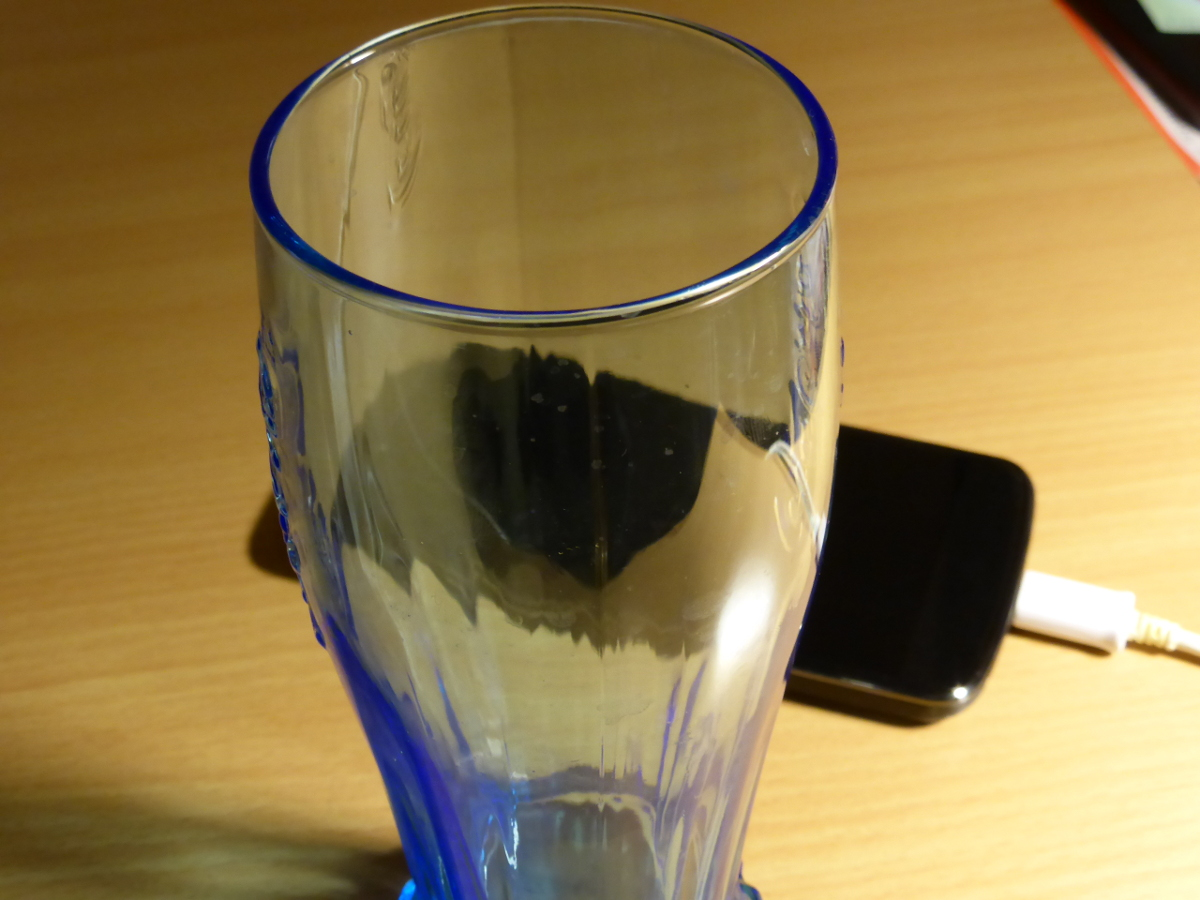
\includegraphics[width=0.6\textwidth]{../images/glass-smartphone-table-2.jpg}
    \end{center}
\end{frame}

\begin{frame}{Taxonomie: Daten}
    \begin{itemize}
        \item Grau oder Farbig?
        \item Tiefeninformation?
        \item Einzelbilder, Stero-Bilder oder Co-Segmentierung?
        \item 2D oder 3D?
    \end{itemize}
\end{frame}

\begin{frame}{Taxonomie: Betriebsart}
    \begin{itemize}
        \item aktiv
        \item passiv
        \begin{itemize}
            \item interaktiv
            \item vollautomatisch
        \end{itemize}
    \end{itemize}
\end{frame}

\begin{frame}{Hier:}
    \begin{itemize}
        \item Klassen: Beliebig, aber meist ohne \texttt{void}.
        \item Pixelzugehörigkeit: Genau eine Klasse pro Pixel.
        \item Daten:
        \begin{itemize}
            \item grau oder farbig
            \item keine Tiefeninformationen
            \item Einzelbilder
            \item 2D
        \end{itemize}
        \item Betriebsmodus:
        \begin{itemize}
            \item passiv, vollautomatisch
        \end{itemize}
    \end{itemize}
\end{frame}
